\documentclass{article}
\usepackage[margin=1.0in]{geometry}

\usepackage{amsmath}
\usepackage{amsfonts}
\usepackage{amssymb}
\usepackage{graphicx}
\usepackage[hidelinks]{hyperref}
\usepackage{lineno}
\usepackage{booktabs}

\usepackage{graphicx}
\usepackage{caption}
\usepackage{subcaption}
\usepackage{hyperref}

\usepackage{listings}
\usepackage{xcolor}

\colorlet{punct}{red!60!black}
\definecolor{background}{HTML}{EEEEEE}
\definecolor{delim}{RGB}{20,105,176}
\colorlet{numb}{magenta!60!black}

\lstdefinelanguage{json}{
    basicstyle=\normalfont\ttfamily,
    %numbers=left,
    %numberstyle=\scriptsize,
    %stepnumber=1,
    numbersep=8pt,
    showstringspaces=false,
    breaklines=true,
    %frame=lines,
    %backgroundcolor=\color{background},
    literate=
     *{0}{{{\color{numb}0}}}{1}
      {1}{{{\color{numb}1}}}{1}
      {2}{{{\color{numb}2}}}{1}
      {3}{{{\color{numb}3}}}{1}
      {4}{{{\color{numb}4}}}{1}
      {5}{{{\color{numb}5}}}{1}
      {6}{{{\color{numb}6}}}{1}
      {7}{{{\color{numb}7}}}{1}
      {8}{{{\color{numb}8}}}{1}
      {9}{{{\color{numb}9}}}{1}
      {:}{{{\color{punct}{:}}}}{1}
      {,}{{{\color{punct}{,}}}}{1}
      {\{}{{{\color{delim}{\{}}}}{1}
      {\}}{{{\color{delim}{\}}}}}{1}
      {[}{{{\color{delim}{[}}}}{1}
      {]}{{{\color{delim}{]}}}}{1},
}

\linenumbers

\newcommand{\median}{\operatorname{median}}

% http://bytesizebio.net/2013/03/11/adding-supplementary-tables-and-figures-in-latex/
\newcommand{\beginsupplement}{%
        \setcounter{table}{0}
        \renewcommand{\thetable}{S\arabic{table}}%
        \setcounter{figure}{0}
        \renewcommand{\thefigure}{S\arabic{figure}}%
     }

\hyphenation{Ge-nome Ge-nomes hyper-mut-ation through-put}

\title{Phage Immuno-Precipitation Sequencing (PhIP-Seq) Pipeline to characterize antibody targets for SARS-CoV-2}
\author{Jared G. Galloway}

% QUESTION: Where should we squeeze in phage-dms explanation? discussion?

\begin{document}
\maketitle

\begin{abstract}
The adaptive immune system interacts and identifies pathogens in the body by identifying a "molecular key" unique to that pathogen.
When an individual is exposed to the pathogen, a full adaptive immune responce can generate a surpluss of antobodies which can bind specifically to that key.
Identifying this molecular key for pathogens of interest remains an outstanding problem crutial to designing vaccines. 
Phage Immuno-Precipitation Sequencing (PhIP-Seq) is a powerful protocol for investigating potential antibody targets (epitopes) \cite{Larman2011}. 
Concretely, this workd by investigating protein-protein interactions between the human body's own antibodies with artificial epitopes displayed on phages (phage vectors).
The key assumption being that recovered patients who have undergone 
a full adaptive response to a disease we care about will have high enough volumes of antibodies (IgG content) to accurately observe an interaction with the pathogen causing the disease. 
Here, we provide and explore two related computational tools created for this data;
(1) An analysis pipeline that takes in demultiplexed next generation sequencing files and produces a coherent dataset to explore the data.
(2) A python package, dubbed \textbf{phippery}, to query this dataset.
Finally, we demostrate the use of this pipeline by applying it to SARS-CoV-2 dataset.
\end{abstract}

\section*{Introduction}

The immune system is most simply divided into two biological mechanisms which we call the innate and adaptive immune systems.
The innate immune system primarily made of cells, such as leukocytes, which can primarily clasify an object as either foreign or native to the body.
this allows for the body to repond quickly to pathogens and invokes reponses that are non-specific to the pathogen it is responding to.
If the pathogen survives these initial attacks, the body's second wave of defence is a more specifc attack known as the adaptice immune responce.
The adaptive immune responce relies upon generating antibodies which can identify a singular pathogen which induced the response. 
Antobodies are used primarily to tag a pathogen which will can then signal a specialized cell, such as a natural killer cell (NKC) to destroy the pathogen. 
Perhaps the most amazing part of the adaptive immune system is the ability to remember a pathogen it has encountered in the lifetime of the host organism.
The ability to rapidly respond to the same pathogen is known as immunity.
 
When designing a vaccine for a specific virus, the memory of the adaptive immune system is leveraged by provoking the immune respose with a 
nuetralized representation of the virus.
This needs to be similar enough to the real virus that it allows the body to generate the right cell machinery,
and obviously without causing real harm to the individual.

Perhaps the largest obsticle when designing vaccines is the genration of a neutral pathogen that accurately embodies the features of the real virus.
To do this, it is often necessary to understand the molecular key -- a peptide chain -- which antibodies use to bind to the pathogen and tag it for later destruction.
Identifying this protein, often referred to as the epitope, remains a large challenge in the field. 
Knowing that the oligonucleotide sequence encoding for this protein lives somewhere where in the genome of the pathogen,
researchers can leverage Next Generation Sequencing (NGS) and Synthetic Oligonucleotide Generation (SONG)
to display a large range of possible epitopes on the surface of a phage.
Those phages are then exposed to antibodies from recovered patients and protein interactions are explored using novel technique known as 
Phage Immuno-Precipitation Sequencing (PhIP-Seq) \cite{Larman2011}.

The PhIP-Seq protocol first requires that a research design a peptide library from a set of pathogen genome loci of interest.
The libraries are most commonly generated by a sliding window across a locus producing oligonucleotide ``tiles" encoding for a peptide.
The size and stride of the nucleotide tiles is designed using specialized software before they are synthesized.
These nucleotide chains are then cloned into a phage with the hope that it models the potential molecular key on the surface of a pathogen. 
When mixed with antibodies, phages-inserted oligos that have binded with an antibody are ``precipitated" out of the mixture using magnetic beads.
The key idea being that the reptoire of phages caught on the beads should then be representitive of antibody targets from the sample.
The samples themselves can come from a variety of sources and individuals most fitting to the experiment being run. 
% TODO conformational vs linear epitope.

Using Next generation sequencing, 
researchers can then quantify the number of phages caught on the beads using barcshort read alignment. 
The analysis of these datas consists demultiplexing the samples,
then aligning the peptides to the reference library in order to generate a count of each specific peptide and sample combination. 
The final result is in the form of a matrix, $X$, where (heuristically) there is a row, $i$, for each peptide and a column, $j$, for each sample.
Concretely, $X_{j,i} =$ the number of reads from sample $i$, which contain the peptide $j$.

Doing analysis for this protocal presents two challenges:
(1) This protocal requires an immense amount of book-keeping and computational power to produce coherent results.
(2) From this protocol, there are a variety of sources from which one can expect add noise to the resulting data, t
hese are including but not limited to; 
IgG content of a sample, "immuno-dominant" antibodies, sequencing bias (GC-content?), amplification bias, and phage display (total amount of each phage in the phage library). 
Here, we describe a pipeline we constructed to handle all bookkeeping and can run the alignment and counts merging steps in parallel to produce a coherent counts matrix with metadata for each sample and peptide.
Additionally, we provide some preliminary results analyzing the output from this pipeline using a python package, \textbf{phippery}, specifically designed for the output of the pipeline.

\section*{Methods}

In data science, a pipeline is a defined set of data processing steps to be run in sequence. 
Pipeline managers such as \textbf{Snakemake} and \textbf{Nextflow} compile the dependencies of one process to the next based on the input. 
Ultimitely this result in a Directed Acyclic Graph (DAG) of data processesing steps and their respective execution order \cite{Merkel_2017, Koster2012}. 
The nature of sample alignments to the peptide encoding oligo sequence reference library makes this a perfect candidate for a workflow manager which can perform these steps in parallel on a high performance computer (HPC). 
For this specific pipeline we use Nextflow paired specialized docker containers to produce a reproducible and highly-parallized workflow \cite{Merkel_2017, DiTommaso2017}.
Nextflow is primarily defined by a set of \textit{Processes}, \textit{Channels}, and \textit{Operators}.
Each Process defined a singular data processing step, given some inputs, using either a command line script or one of few popular data-driven programming languages.
Further, each process execution is run in a containerized environment where the inputs are staged in an independent temporary directory.
In other words, the pipeline manager handles all process input and output through \textit{Channels} so the individual processes don't conflict with each other in terms of file system or necessary software dependencies.
A \textit{Channel} can be thought of as a First-In-First-Out (FIFO) queue and act as the only mode of communication between the data processing steps.
Processes which define their input from a channel are executed as soon as something is put in the queue.
\textit{Operators} allow us to merge, split, or transform the items placed in a channel to configure a nicely formatted output usually containing files and metadata
needed for a downtream process.
Figure \ref{fig:DAG} shows the DAG of our pipeline from input metadata and sequencing file to a specialized python object containing
the repective counts and metadata for each sample and peptide \cite{van1995python}.
In this section, we will discuss the pipeline inputs, the individual steps of the pipeline, and the resulting output.

\begin{figure}[h!!!!]
\centering
    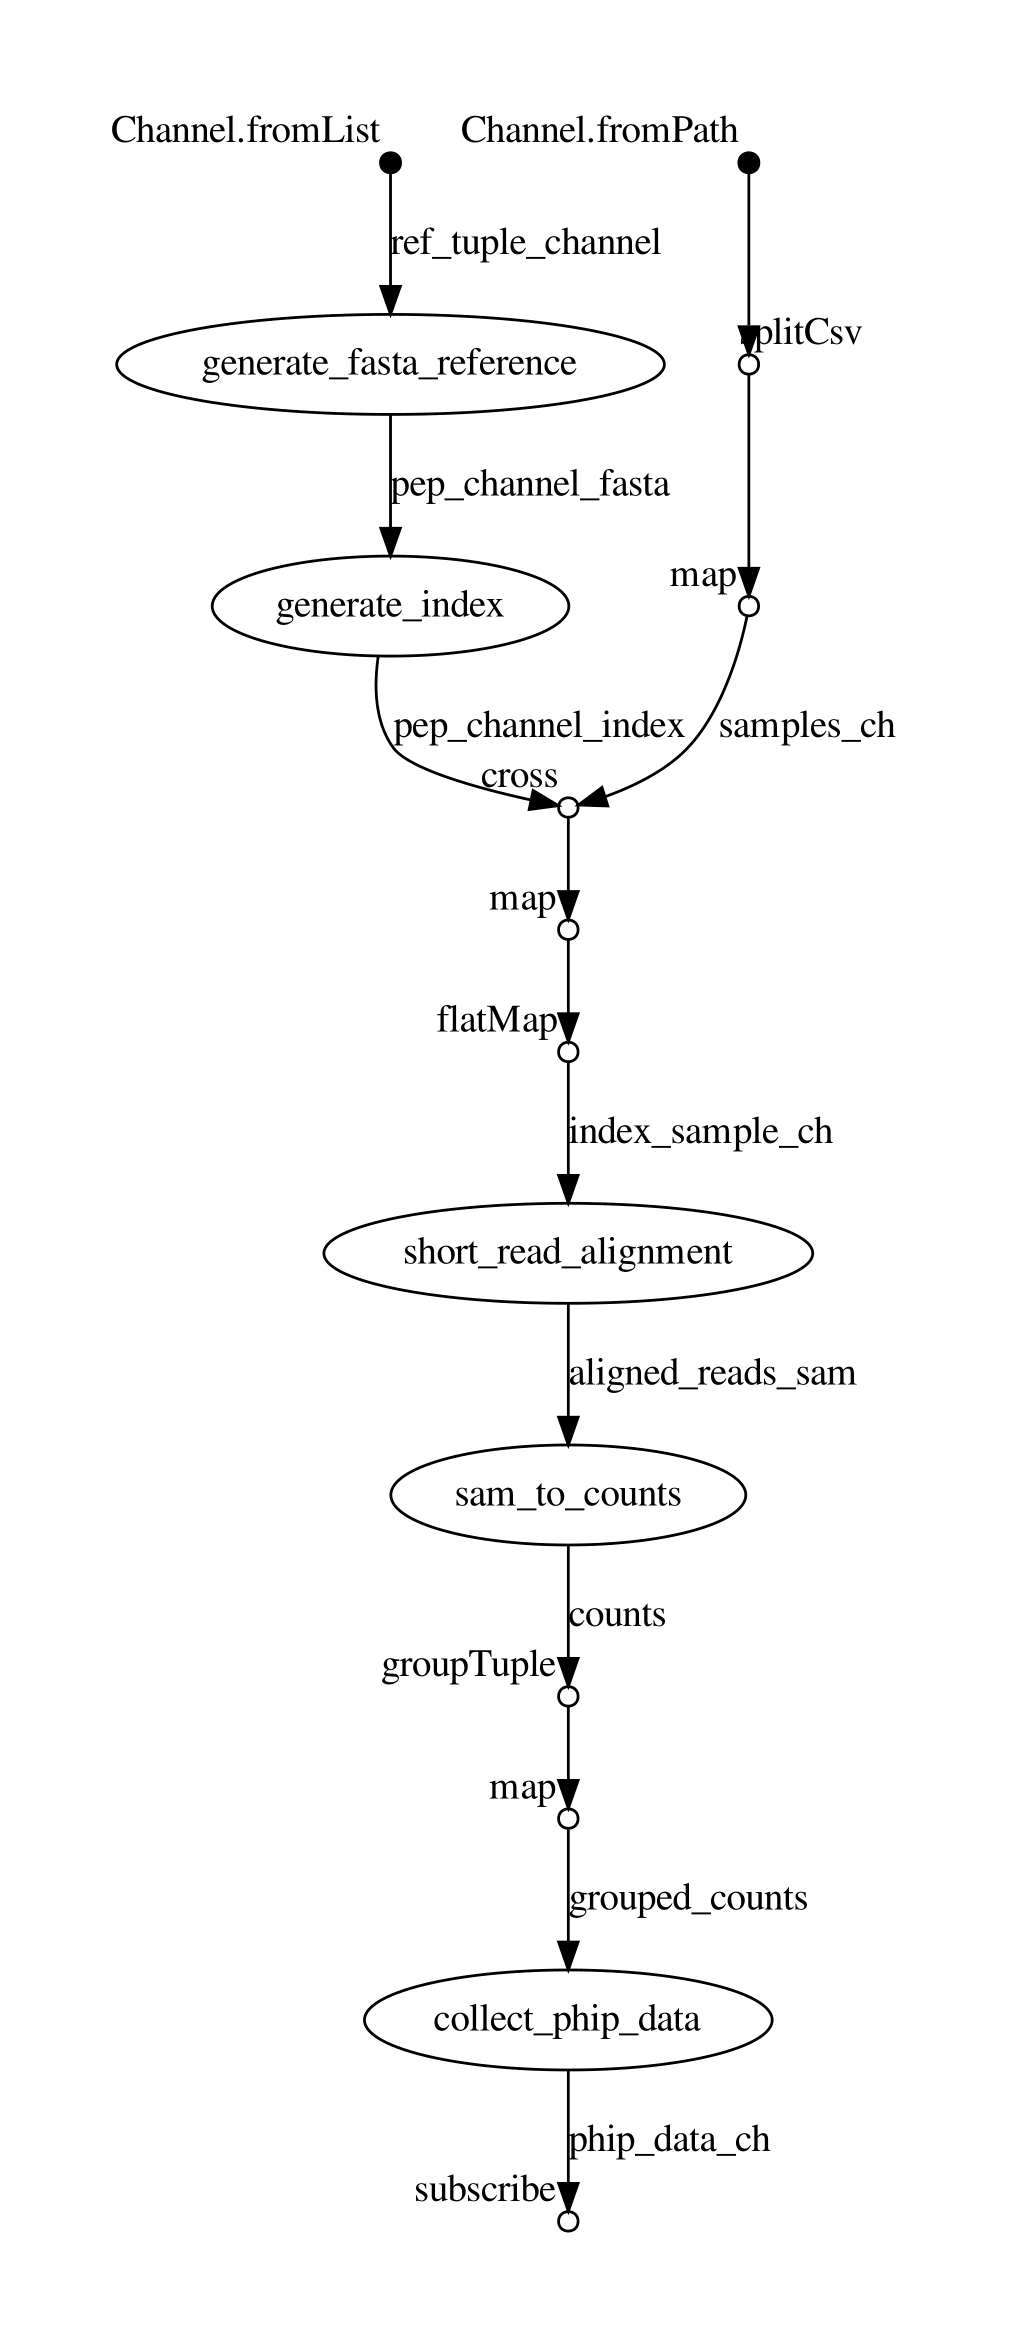
\includegraphics[width=0.5\textwidth]{figures/dag-1.png}
    \caption { \
The Directed Acyclic Graph (DAG) representation of our pipeline workflow. 
Here, each bubble represents a single data processing step to be run in temporary directory inside a respective docker container. 
The arrows specify \textbf{Nextflow} ``channels" which direct and organize output from one process to the next. 
Dots between channel arrows specify where a \textbf{Nextflow} ``operator" was used to organize and collect the output of a set of channels into another set of channels.
}
\label{fig:DAG}
\end{figure}

\subsection*{Pipeline Input - Data}

To configure the run of a pipeline the user must specify the path of JSON configuration file.
This file contains information about where the pipeline can find sample and peptide metadata, 
the sample fastq files for each experiment, and some information about read and reference oligo length. 
Using this, the pipeline automatically parses the JSON file and configures the steps needed to generate the output.
This approach allows the user to organize their data how they like, and let the pipeline handle everything else.

\paragraph{config file}
There a few key-value pairs that are required to be in the configuration file. 
An example configuration file for a simulated dataset is shown in Listing \ref{listing:config.json}.
First the user must specify an ``output\_dir" key with the value as a filepath where the would like the results of the pipeline to be published.
In general, the pipeline outputs itermediary files organized by reference, experiment, and PhipData Object output.
under the specified output directory. The ``samples" key must specify a valid path to a sample metadata csv descibed below. 
Each sample is tied directly to one of the keys specified in ``experiments", 
and so for each experiment you expect to see across the samples being run, a path to the directory containing the sample fastq 
Similarly, each sample specifies a reference library it should be aligned against.
The ``reference" key specifies a filepath for each peptide metadata file defining the reference index to be built during the pipeline run.
Additionally, there are a few other parameters which can be used to specify read and reference oligo length for alignment schemes.
It should be clear that only a \textit{single} sample metadata csv is specified, while \textit{multiple} peptide references can be specified.
The pipeline will output a phippery PhipData object for each reference each containing the respective samples as descibed in the sample metadata file.

\begin{lstlisting}[language=json,firstnumber=1,caption={An example JSON configuration file for a simulated dataset.},captionpos=b,numbers=none,label=listing:config.json]
{
    "output_dir" : "simulate_ones/",

    "samples" : "simulate_ones/samples/sample_metadata.csv",

    "experiments" : {
        "expa" : "simulate_ones/experiments/expa/some/path/",
        "expb" : "simulate_ones/experiments/expb/some/path/"
    },

    "references" : {
        "refa" : "simulate_ones/references/peptide_metadata_a.csv",
        "refb" : "simulate_ones/references/peptide_metadata_b.csv"
    }
}
\end{lstlisting}

\paragraph{Sample metadata}
To specify which samples are to be included in the pipeline run, 
the researcher who designs the experiment compiles a comma-seperated file specifying all relevent metadata for each Immuno-Precipitation experiment run. 
Table \ref{tab:sample_metadata} shows an example of this sample metadata table for simulated data.
There are four required fields that must be specified for each sample (row) in the file;
(1) A unique indentifier in the form of a single integer, specified in the ``ID" column.
(2) The file \textit{pattern} which specifies the filenames for all technical replicates of a single sample in the ``fastq\_pattern" column.
(3) An ``experiment" name which, in the config file, ties the sample to the location of the base directory where the fastq file is expected to be found.
(4) A ``reference" name which speifies the index the samples should be aligned to.
While the are the only \textit{required} fields it's generally useful to add any other relevent metadata connected to each sample such as sample type, species etc.
Any and all fields can be useful for downstream analysis when querying the dataset. 

\begin{table}[h!!!!]
\centering
\begin{tabular}{llll}
\toprule
{} &           fastq\_pattern & reference & experiment \\
ID &                         &           &            \\
\midrule
0  &              sample-*-0 &      refa &       expa \\
1  &              sample-*-1 &      refa &       expa \\
2  &  xeno-AE-122-*-R1.3.3.0 &      refa &       expa \\
3  &  xeno-AE-122-*-R1.3.3.1 &      refa &       expa \\
4  &  xeno-AE-122-*-R1.3.3.2 &      refa &       expa \\
5  &  xeno-AE-122-*-R1.3.3.3 &      refb &       expb \\
6  &  xeno-AE-122-*-R1.3.3.4 &      refb &       expb \\
7  &          johnny-boy-*-0 &      refb &       expb \\
8  &          johnny-boy-*-1 &      refb &       expb \\
9  &          johnny-boy-*-2 &      refb &       expb \\
\bottomrule
\end{tabular}
\caption{An example sample metadata table containing the requires fields for a simulated dataset.}
\label{tab:sample_metadata}
\end{table}

\paragraph{Peptide metadata}
For each unique reference listed in sample metadata file, we must specify a peptide metadata comma-seperated file
in order to build an index for the sample to be aligned against and identify which peptide, if any, a sample read aligns to.
As seen in Table \ref{tab:peptide_metadata}, there only two required fields;
(1) A unique indentifier in the form of a single integer, specified in the ``ID" column.
(2) the ``Oligo" column specifying the nucleotide encoding for a specific peptide. 
Currently, we expect the index oligo sequences, if there at all, be lowercase, and the peptide encoding sequence be uppercase.
Similarly to the sample meadtata table, it is generally useful to include other information about the peptide such the virus
strain, and some genomic positional information.

\begin{table}
\centering
\begin{tabular}{ll}
\toprule
{} &                                              Oligo \\
ID &                                                    \\
\midrule
0  &  gcatcagtaggctgcgtaGGGATTAGGCGGACCTCCATGAATACCG... \\
1  &  gcatcagtaggctgcgtaTGTAGGCAAGGAGCAACACTTCTTCTTT... \\
2  &  gcatcagtaggctgcgtaGAGAATGGGCCAGGAATGATCTACTGTC... \\
3  &  gcatcagtaggctgcgtaCGTGTCAAAAACTGCGTATTTACGAAGA... \\
4  &  gcatcagtaggctgcgtaTTTCAGATCCTACCATTTGTGTCCTTAA... \\
5  &  gcatcagtaggctgcgtaCCGAGTTCGTATTTTTACAAATCCCGGA... \\
6  &  gcatcagtaggctgcgtaTATTTAATGAGTGTGAGGCAAAGTTGTT... \\
7  &  gcatcagtaggctgcgtaTTTACGCTCAGCAAGCGTAGCTAGCATG... \\
8  &  gcatcagtaggctgcgtaTCAAACAGGTTACGACACAAAGAACGCC... \\
9  &  gcatcagtaggctgcgtaTCGCATTCTCCTGGCCTACTTACAGTTC... \\
\bottomrule
\end{tabular}
\caption{An example peptide metadata table containing the requires fields for a simulated dataset.}
\label{tab:peptide_metadata}
\end{table}

\subsection*{Data Processing Steps}

There are a number of individual data processing steps that take place when running this pipeline.
The number of times each process is run is determined by the number of references and samples.
Concretely, if there are $S$ samples, each with $T$, in the sample metadata table, and $R$ references then we can expect $2ST + 3R$ separate processes to be run. 
In this section, we will briefly review the unique data processing steps in the pipeline.
The pipeline begins by defining two input channels; 
the first channel defines the references to be generated and their respective peptide metadata tables from which to generate the index for downstream alignment,
the second channel parses each sample in the sample metadata file, finds all technical replicates for that sample, and merges with the first channel before sequence
alignment, counts generation, and counts merging. 

\paragraph{generate fasta reference}
The first step in the pipeline is to parse the configuration file for all listed references and respective peptide metadata files. 
For each reference found, the pipeline executes a ``generate\_fasta\_reference" process.
The primary job for this step is to produce a fasta representation of the respective peptide metadata table in preparation for index generation.
Simply put, this step simply converts the ID into a header followed by the oligo sequence for each peptide in the table.
A container for the \textbf{phippery} python package is used as the primary execution step.
For cluster submission, we request only a single core with a modest amount of memory since the software being used isn't multithreaded.

\paragraph{Index generation}
For samples to be aligned to the reference, a specific binary index must be generated.
In this step, we use \textbf{bowtie-build} to generate the index which each respective sample will be aligned to \cite{Langmead2009}
The five binary files that are output are nested in a subdirectory dir named ``<reference name>\_index".
This process is run in a public \textbf{bowtie} container hosted on Quay and \textit{can} be multithreaded. 

\paragraph{Short read alignment}
The bulk of the work performed in the pipeline happens during short-read sequence alignment of every technical replicate to it's respective reference peptide library.
After the the references have been built and the sample metadata file has been parsed, we merge the channels into a new channel, named \textit{index\_sample\_ch}.
This channel is a queue which outputs an array containing 

\subsection*{Pipeline Output}



\section*{Preliminary Results on an Anonymous Dataset}

The pipeline described above has thus far been used on a novel set of empirical datasets and produced note-worthy results.
However, due to this being unpublished and private data, we will not be including any defining names or details of the experiment.
Instead, we will simply present the figures and explain what they are excluding virus strain names and result interpretations.

$\approx 1 page$

1. Introduce phippery and 

\begin{figure}[h!!!!]
\centering
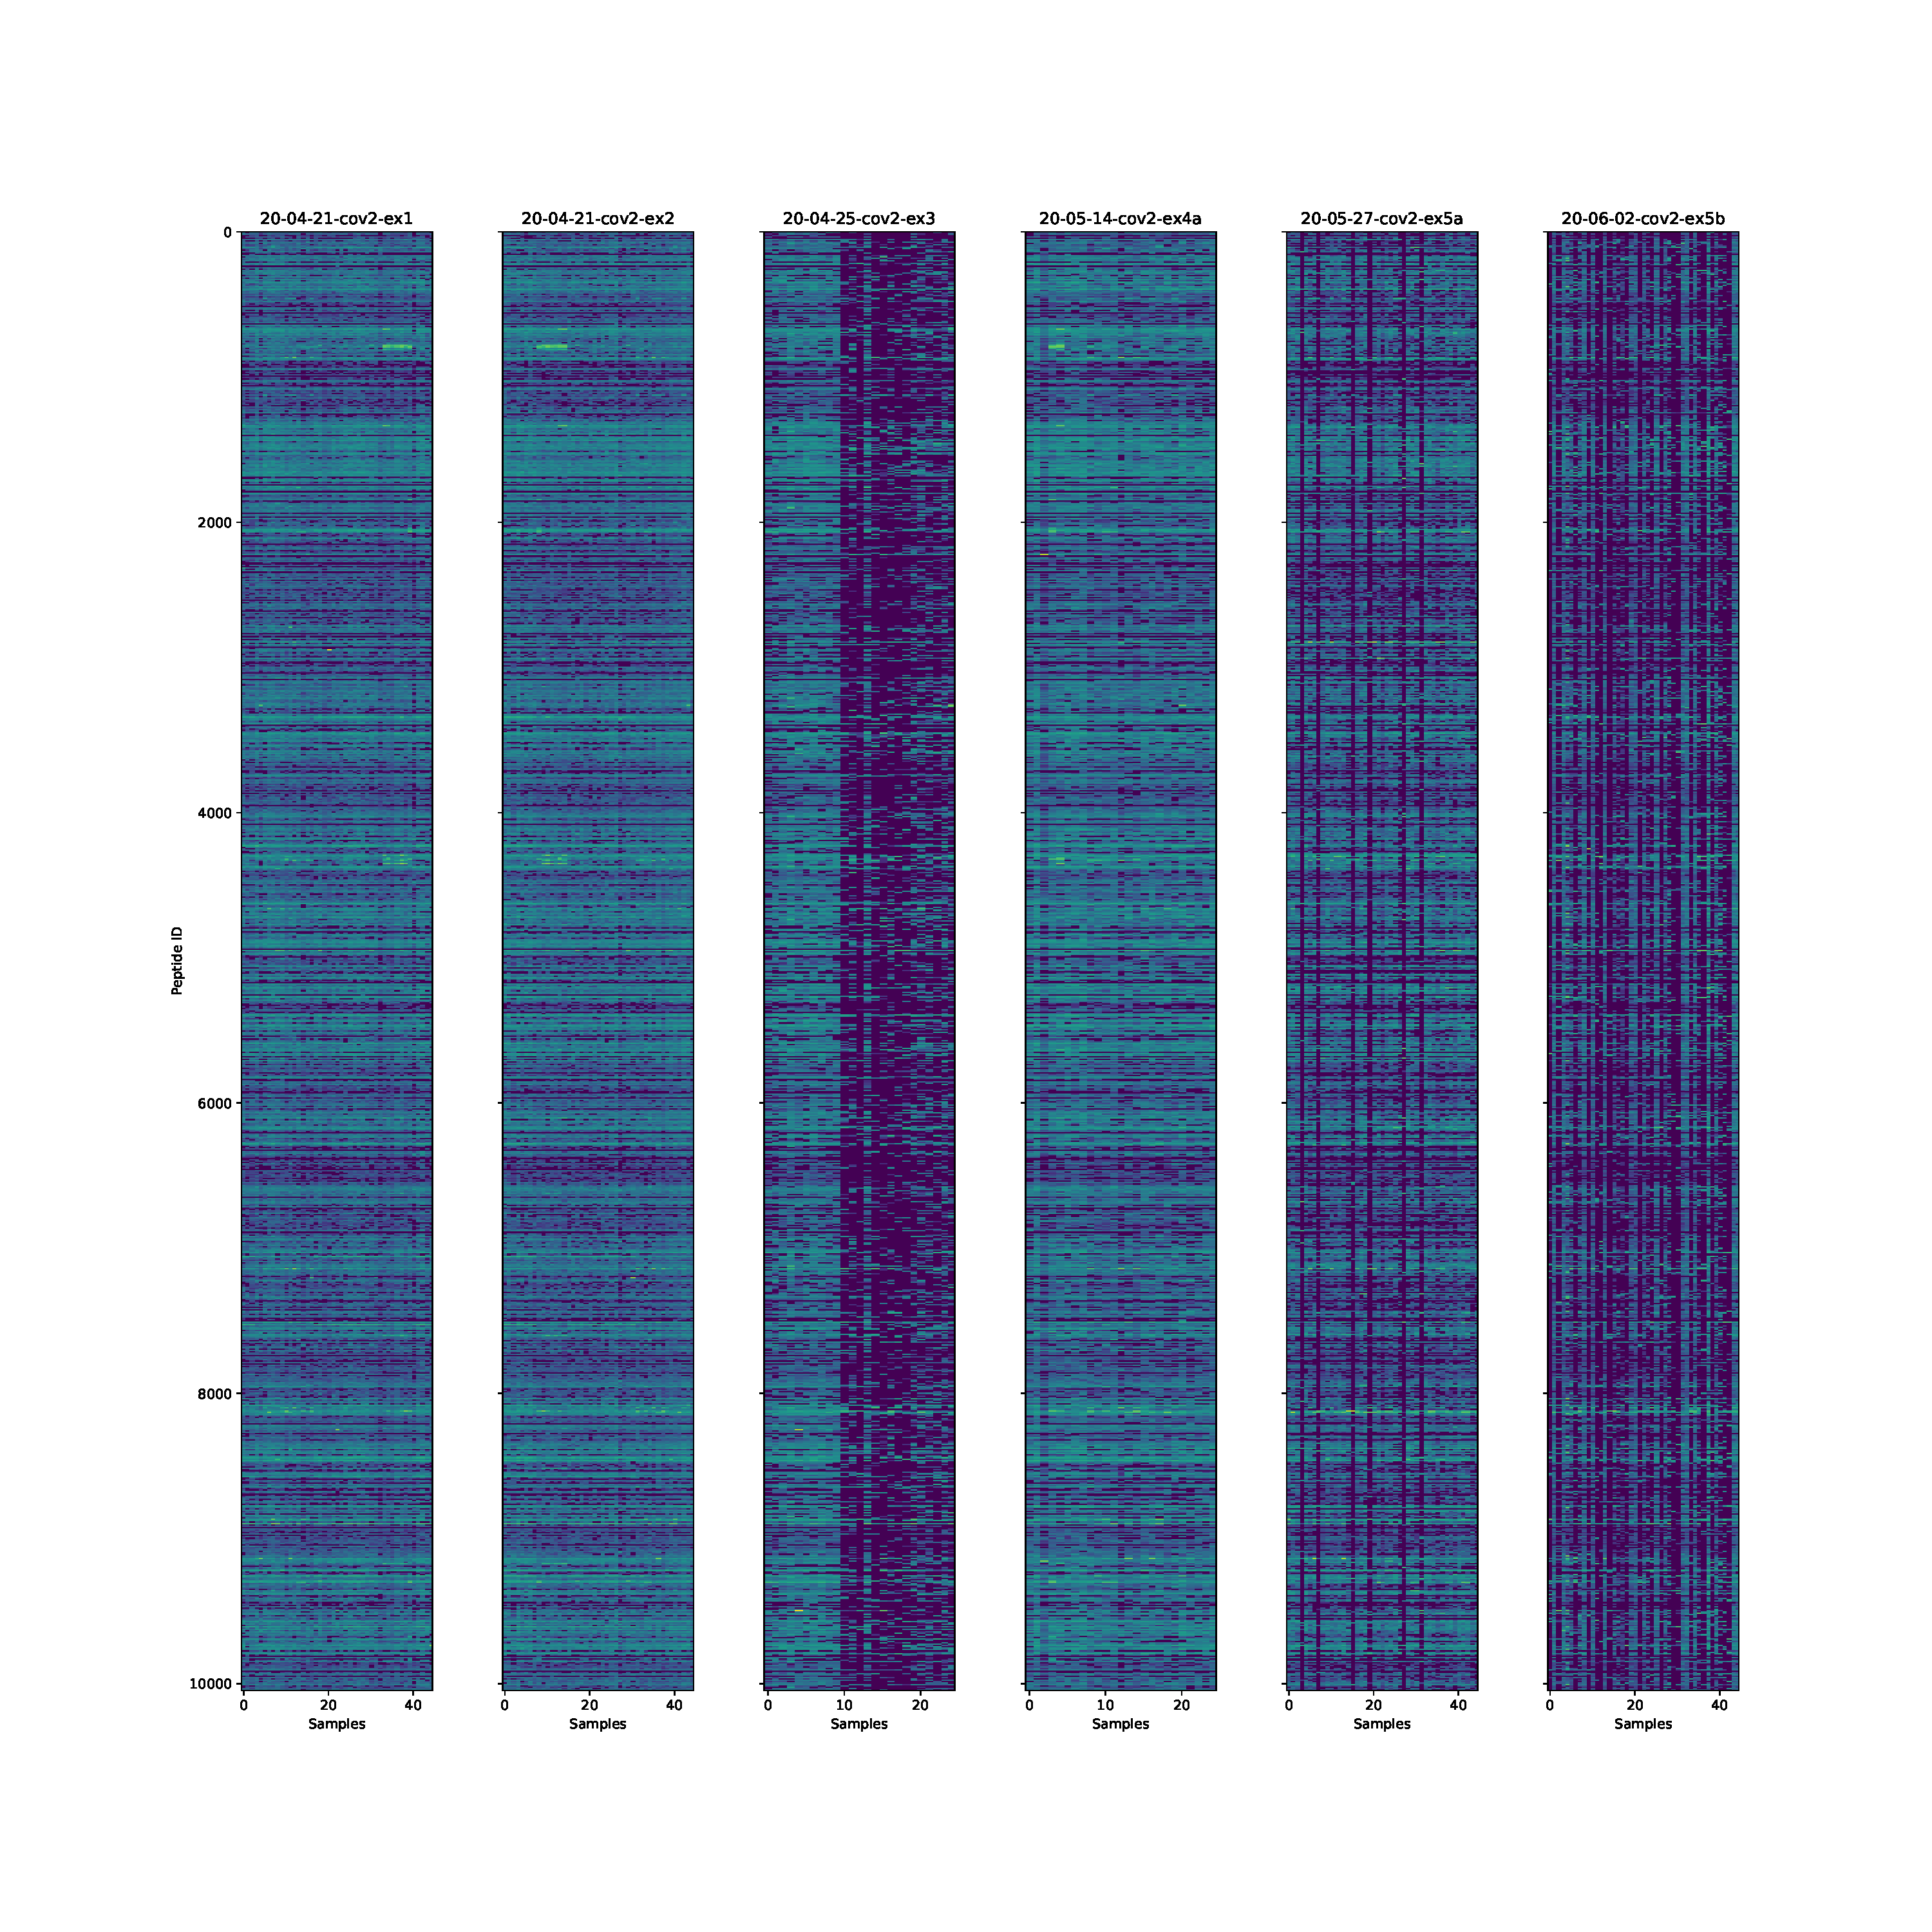
\includegraphics[width=1.0\textwidth]{figures/raw_counts.pdf}
\caption{ \
Raw counts.
}
\label{fig:raw_counts}
\end{figure}

\begin{figure}[h!!!!]
\centering
\includegraphics[width=1.0\textwidth]{figures/correlation_by_experiment_sample_type.pdf}
\caption{ \
Technical Replicates
}
\label{fig:tech_reps}
\end{figure}

\bibliographystyle{plain}
\bibliography{main}

% \clearpage
% \section*{Supplementary Materials}
% \beginsupplement
% Supplementary text and figures here.

\end{document}




